%------------------------------------------------

\begin{fullwidth}

% What is data cleaning
Raw data files may be received in a variety of formats,
and are often not immediately suited for use with statistical software.
This chapter describes the workflow of preparing newly-acquired data for analysis.
The tasks described in this chapter have many different names:
data cleaning, data munging, data wrangling.
But they all mean the same thing --
transforming raw data into a convenient format for your intended use.
This is the most time-consuming step of a project's data work,
particularly when primary data is involved;
it is also essential for data quality.
This chapter outlines the workflow our team developed to make the process efficient and transparent.
One key point of this chapter is that no changes are made to the contents of data at this point.
We consider creating new variables, imputing values and correcting outliers
to be research decisions, and will discuss those in the next chapter.
Therefore, the clean dataset,
which is the main output from the workflow discussed in this chapter,
contains almost exactly the same information as the raw data,
but in a format that is ready for use with statistical software.

% Chapter overview
This chapter describes the various tasks involved in making newly-acquired data ready for analysis.
The first section will show how to make your data \textit{tidy}.
This means adjusting how the dataset is organized
until the relationship between its rows and columns is well-defined.
The second section describes quality assurance checks,
which are necessary to verify the accuracy of your data.
After that, identifying information is typically no longer needed;
therefore the third section outlines steps to remove direct identifiers.
Finally, the last section discusses how to examine each variable in your dataset and
make sure that it is as well documented and as easy to use as possible.
One important thing to take note is that all these tasks are implemented through code,
and resulting datasets are saved in new files that can be reproduced by running this code.
The raw data files are kept exactly as they were acquired,
and no changes are made directly to them.

\end{fullwidth}

%------------------------------------------------


\section{Making data ``tidy''}

% Intro
The very first step in creating an analysis-friendly dataset
is understanding the data acquired,
and using this understanding to translate the data into an intuitive format.
This section discusses what steps may be needed to make sure that each row
in your \textbf{data tables}\sidenote{\textbf{Data table:}
	data that is structured into rows and columns.
	Also called \textit{tabular datasets} or \textit{rectangular data}.
	Examples of non-rectangular data are written text,
	NoSQL and graph databases, or files such as images.}
represents one observation.
Getting to such a format may be harder than expected,
and the \textbf{unit of observation}\sidenote{\textbf{Unit of observation:}
	the unit described by the data. In datasets, it is ideally what each row represents.
  \url{https://dimewiki.worldbank.org/Unit_of_Observation}}
 may be ambiguous in many raw datasets.
This section will present what we call a \textit{tidy} data format,
which is, in our experience, the ideal format to handle tabular data.
Although this may at first seem out of place, as it comes before quality assurance,
we believe that this is the appropriate first step in data cleaning,
that it should be done continuously as data is recieved,
and that quality assurance is best done using tidied data.

\begin{fullwidth}
	\begin{figure}
		\centering
		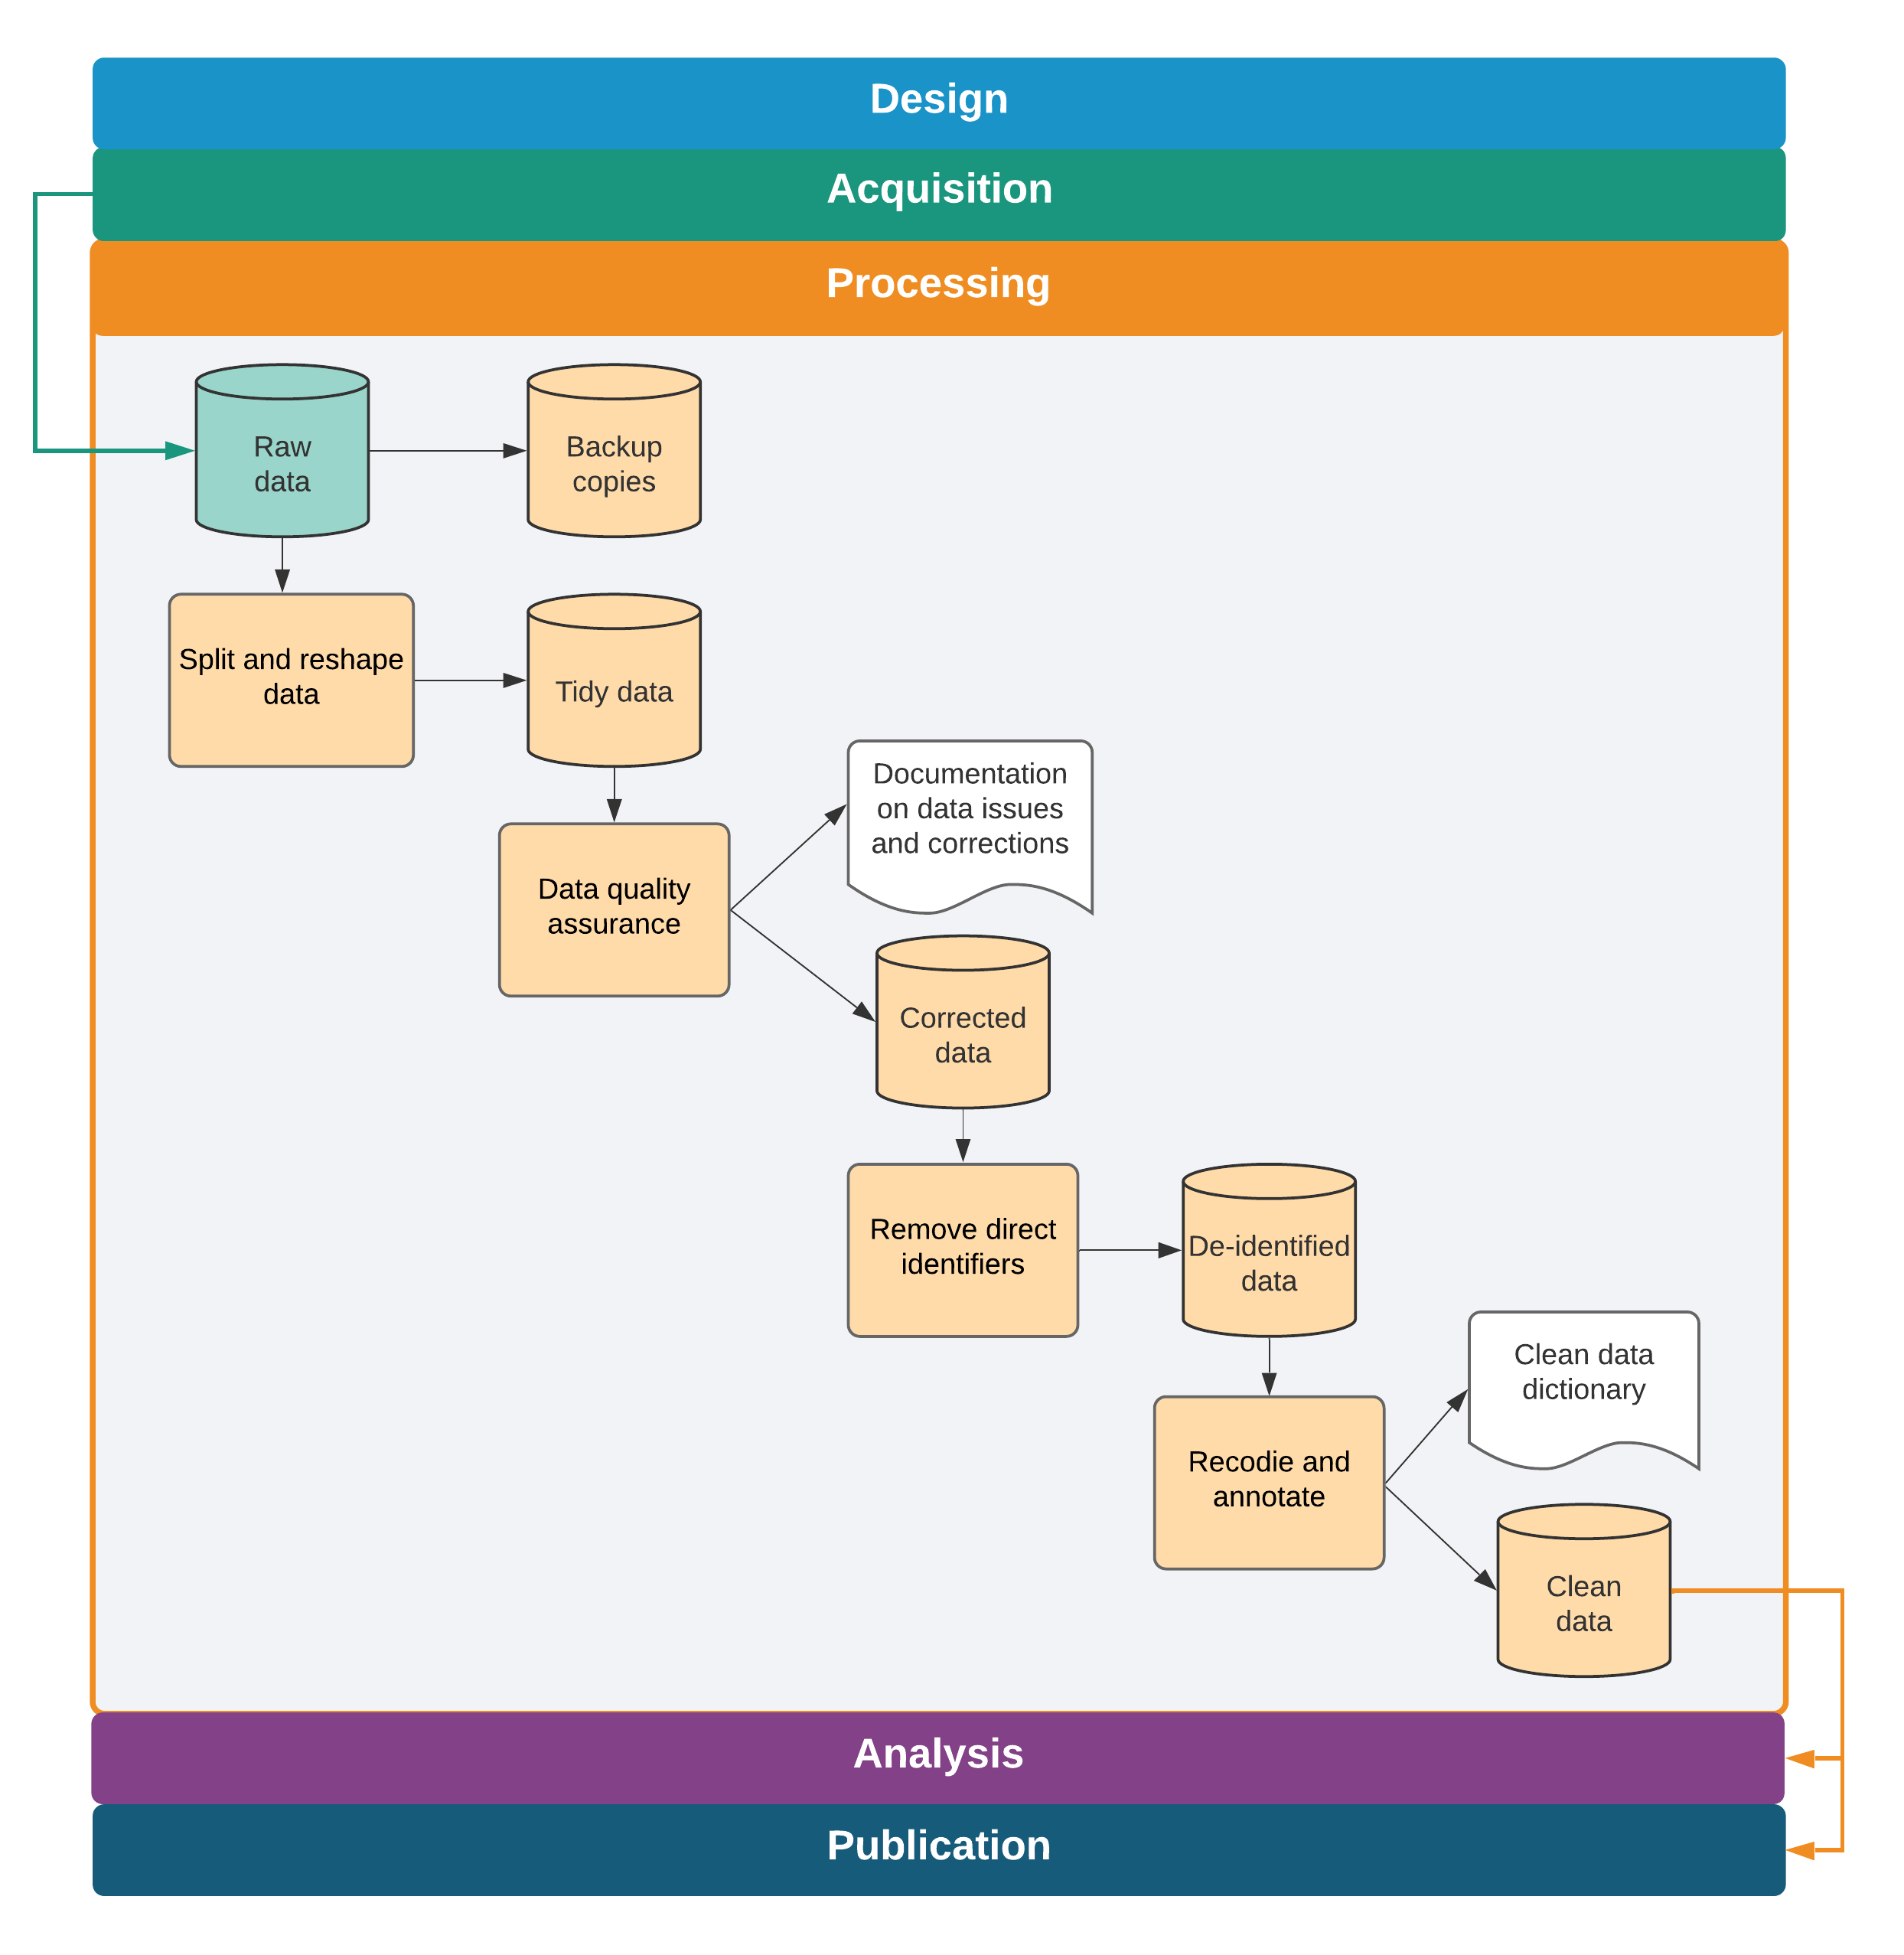
\includegraphics[width=1.6\linewidth]{diagrams/Cleaning}
		\caption{}
		\label{fig:intro}
	\end{figure}
\end{fullwidth}

%------------------------------------------------------------------------------
\subsection{Unique identifiers}

% Uniquely and fully identifying variable
An important step before starting to tidy a dataset is
to understand the \textbf{unit of observation}\sidenote{
	\textbf{Unit of observation:} the unit described by the data.
	In a data table, it is what each row represents.
  \url{https://dimewiki.worldbank.org/Unit\_of\_Observation}}\index{unit of observation}
and find out which variable or set of variables is the \textbf{unique identifier}\sidenote{
  \url{https://dimewiki.worldbank.org/ID\_Variable\_Properties}}\index{unique identifier}
for each observation.
Ensuring that observations are uniquely and fully identified
is arguably the most important step in data cleaning.
It may be the case that the variables expected to uniquely identify
the raw data contain either missing or duplicate values.\sidenote{
	We use the expression \textbf{raw data}
	to refer to both ``data in the state it was originally received by the research team''
  as well as to ``corrected and compiled datasets created from received information,
  reflecting only that information'',
  depending on the context.
	This applies to data acquired from partners as well as
	primary data collected by the research team.}
It is also possible for a raw dataset to not include a unique identifier,
or for the identifier to involve a long string
that is difficult to work with, such as a person's name.
In such cases, cleaning begins by either carefully creating a variable
that uniquely identifies the data,
or merging the ID variable from the master dataset
using other identifying information.
Note that while digital survey tools create unique identifiers for each data submission,
that is not the same as having a unique ID variable for each observation in the sample,
as there can be multiple submissions for the same observation.

As discussed in Chapter 3,
the unique identifier will be used to link observations in this dataset
to data in other data sources according to the \textbf{data linkage table},\sidenote{
  \url{https://dimewiki.worldbank.org/Data_Linkage_Table}}\index{data linkage table}
and all observations must be listed in the \textbf{master dataset}.\sidenote{
	\url{https://dimewiki.worldbank.org/Master\_Data\_Set}}\index{master dataset}
Part of the process of understanding the level of observation in a dataset
and finding or creating its unique identifier is to
make sure that each observation is represented in the master dataset by a unique ID value.
If you encounter any observations that are not listed in the master dataset,
you should assign them a unique ID and add them to the master dataset.
Always convince yourself beyond reasonable doubt that the new observation
is indeed a new observation,
and not one that is already listed, only with a different ID value.

DIME Analytics created an automated workflow to identify, correct and document
occurrences of duplicated entries in the unique identifier using
\texttt{ieduplicates} and \texttt{iecompdup},\index{\texttt{ieduplicates}}\index{\texttt{iecompdup}}
two Stata commands included in the \texttt{iefieldkit}\index{\texttt{iefieldkit}}
package\index{iefieldkit}.\sidenote{\url{https://dimewiki.worldbank.org/iefieldkit}}
One advantage of using \texttt{ieduplicates}\sidenote{\url{
		https://dimewiki.worldbank.org/ieduplicates}}
to correct duplicated entries is that it creates \textit{duplicates reports}
which records each corrections made and documents the reason for it.
Even if you are not using this command,
it is important to keep a record of all cases of duplicated IDs encountered
 and how they were resolved.

%-------------------------------------------------------------------------------
\subsection{Tidying raw data}

Though raw data can be acquired in all shapes and sizes,
it is most commonly received as one or multiple data tables.
These data tables can organize information in multiple ways,
and not all of them result in easy-to-handle datasets.
Fortunately, a vast literature of database management has identified the format
that makes interacting with the data as easy as it can be.
We call data in such format \textbf{tidy}.
A data table is tidy when each column represents one \textbf{variable},\sidenote{
  \textbf{Variable:} the collection of all data points
	that measure the same attribute for each observation.}
each row represents one observation,
and all variables in it have the same unit of observation.
Every other format is \textit{untidy}.
This may seem trivial, but raw data,
and raw survey data in particular,
is rarely received in a tidy format.

The most common case of untidy raw data encountered in development research
is a dataset with multiple units of observations stored in the same data table.
Take, for example, a household survey that includes household-level questions,
as well as a household member roster.
Such raw datasets usually consists of a single data table
where questions from the household member roster are saved in different columns,
one for each member, with a corresponding member suffix,
and household-level questions are represented by one column each.
When your rows include multiple nested observational units,
then the identifying variable does not identify all observations on that row,
as there is more than one unit of observation on the same row.

Survey data containing nested units of observation is typically
imported from survey platforms in \textbf{wide format}.\sidenote{\textbf{Wide data:}
	a data table where a single variable is divided into multiple columns,
	for example one for each individual in a household.}\index{wide data format}
Wide format data could have, for instance,
one column for a household-level variable (for example \texttt{ownsfridge}),
and a few columns for household member-level variables (for example \texttt{sex\_1}, \texttt{sex\_2}).
Raw data is often saved in this format because it's the most efficient way to transfer it:
adding different levels of observation into the same data table
allows for data to be transferred in a single file.
However, this leads to the widespread practice of interacting with data in wide format,
although doing so is often inefficient and error-prone.

To understand how dealing with wide data can be complicated,
imagine you need to calculate the share of women
in each household using the household level data described above.
In a wide data table you will either have to first create variables counting
the number of women and the total number of household members,
and then calculate the share,
or you will have to transform the data to a different format.
In a tidy data table, however, where each row is a household member,
you can easily aggregate the share of women by household,
without additional steps,
and then merge the result to the household-level data tables.
Tidy data tables are also easier to clean,
as each attribute only needs to be checked once,
and each column corresponds directly to one question in the questionnaire.
Finally, as you will see in Chapter 6,
summary statistics and distributions are much simpler
to generate from tidy data tables.

As mentioned earlier, there are unlimited ways for data to be untidy;
wide format is only one of those ways.
Another example is a data table containing both information on transactions
and on the firms involved in each transaction.
In this case, the firm-level information will be repeated
for all transactions a given firm was involved in.
Analyzing data in this format would give more weight
to firms that conducted more transactions,
which may not be consistent with the research design.

The basic process behind tidying a data table is simple:
first, identify all the variables that were measured at the same level of observation;
second, create separate data tables for each level of observation;
and third, reshape\sidenote{\textbf{Reshape:}
	transform a data table in such a way that the unit of observation represented by a row changes.}
the data and remove duplicated rows
until each data table is uniquely and fully identified by the identifying variable
that corresponds to its unit of observation.
Reshaping data tables is the most intricate task in data cleaning;
you should be very familiar with commands such as
\texttt{reshape} in Stata and \texttt{pivot} in R.
You must be sure that identifying variables are consistent across data tables,
so they can always be linked.
Reshaping is the type of transformation we referred to
in the example of how you calculate
the share of women in a wide data set.
The important difference is that
in a tidy workflow,
instead of transforming the data for each operation,
this transformation is done once for all data during cleaning,
making all subsequent operations much easier.

In the earlier household survey example,
household-level variables will be stored in one tidy data table,
and household-member variables are reshaped
and stored in a separate, member-level, tidy data table,
which also contains the household ID for each individual.
The household ID is intentionally duplicated in the household members data table
to allow one or several household members to be linked to the same household data.
The unique identifier for the household member-level data data will be
either a single household member ID or
a combination of household ID and household member ID.
In the transaction data example,
the result of the tidying process would be one transaction-level data table,
containing variables indicating the ID of all firms involved;
and one firm-level data table with a single entry for each firm.
Then, firm-level analysis is easily done
by calculating appropriate statistics in the transactions data table
(in Stata, often through \texttt{collapse})
and then merging or joining those results to the firms data table.

In a tidy workflow, your clean dataset comes from 
a group of one or more tidy data tables.
This is reflected in the data flowcharts from your data map
showing the way to combine data from the master datasets
any any other datasets that you obtained.\index{data flowchart}\index{data map}
In both examples above, your clean dataset is made up of two tidy data tables.
There must be a clear way to connect each
tidy data table to a master dataset,
and thereby also to all other datasets.
To implement this, you need to decide which data table is the main data table;
that data table's unit of observation will be
the main unit of observation of your dataset.
The main unit of observation must directly correspond to a master dataset,
and be listed in the data linkage table.
All other data tables in your dataset must have
an unambiguous way to merge with the main data table.
This way, it will be possible to link
all data points in all your project's datasets to each other.
We recommend that you save your datasets as a folder,
in which the main data table shares the same name as the folder,
and the name of all other data tables start with the same name,
but are suffixed with the unit of observation for that data table.

In the household dataset example,
the household-level data table would be the main table.
This means that there must be a master dataset for households.
(You may have a master dataset for household members as well
if you think it is important for your research,
but it is not strictly required.)
The household data set would then be stored in a folder called,
for example, \texttt{baseline-hh-survey/}.
In that folder you would save both
the household-level data table with the same name as the folder,
for example \texttt{baseline-hh-survey.csv},
and the household member-level data named in the same format but with a suffix,
for example \texttt{baseline-hh-survey-hhmember.csv}.

The tidying process gets more complex as the number of nested groups increases.
That means the steps of identifying the unit of observation of each variable
and reshaping the separated data tables need to be repeated multiple times.
However, the more nested groups a dataset includes,
the more efficient it is to deal with tidy data as compared to untidy.
Cleaning and analyzing wide datasets, in particular,
is a repetitive and error-prone process.

The next step of data cleaning, data quality monitoring,
may involve comparing different units of observation.
Aggregating sub-units to compare to a higher unit is much easier with tidy data,
which is why we suggest tidying data as the first step in the cleaning workflow.
If you are conducting primary data collection,
you can start preparing or coding the data tidying even before the data is acquired,
since you will know in advance the exact format in which the data will be received.
In the case of survey data,
tidying datasets will guarantee a one-to-one correspondence
between questions in the questionnaire and columns in the data.
Preparing the data for analysis, the last task in this chapter,
is much simpler when that is the case.

%------------------------------------------------
\section{Data quality assurance}

% Intro
Whether you are acquiring data from a partner or collecting it directly,
it is important to make sure that data faithfully reflects ground realities.
You should carefully examine and clean any data you are about to use.
When reviewing raw data, you will inevitably encounter data entry mistakes,
such as typos and inconsistent values.
Data quality assurance requires a combination of real-time data checks
and back-checks or validation audits, which often means tracking down
the people whose information is included in the dataset.

\subsection{Implementing high-frequency quality checks}

% What are HFCs
A key advantage of continuous electronic data intake methods,
as compared to traditional paper surveys and one-time data dumps,
is the ability to access and analyze the data acquisition process is ongoing.
Data issues can then be identified and resolved in real-time.
Designing systematic data checks and running them routinely throughout data intake
simplifies monitoring and improves data quality.
To prepare for data acquisition,
the research team should develop a \textbf{data quality assurance plan}.\sidenote{
	\url{https://dimewiki.worldbank.org/Data\_Quality\_Assurance\_Plan}}
While data is being acquired,
a research assistant should work closely with the field team or data licensing partner
to ensure that the data is flowing as expected,
and to set up and perform \textbf{high-frequency checks (HFCs)} with the incoming data.

% Why they should be made in real-time
High-frequency checks should carefully inspect key treatment and outcome variables
to ensure that the data quality of core study variables is uniformly high,
and that additional effort is centered where it is most important.
Data quality checks should be run every time data is received
to flag irregularities in the aquisition progress, in sample completeness, or in response quality.
The faster issues are identified, the more likely they are to be solved.
\texttt{ipacheck}\sidenote{
	\url{https://github.com/PovertyAction/high-frequency-checks}}
is a very useful Stata command that automates some of these tasks,
regardless of the data source.

% Completeness
It is important to check continuously that the observations received match the intended sample.
In surveys, electronic survey software often provides case management features
through which sampled units are directly assigned to individual enumerators.
For data received from partners, such as administrative data,
this may be harder to validate.
In these cases, cross-referencing with other data sources can help to ensure completeness.
It is often the case that raw data includes duplicate or missing entries,
which may occur due to typos, failed submissions to data servers,
or other mistakes.\sidenote{
	\url{https://dimewiki.worldbank.org/Duplicates_and_Survey_Logs}}
Issues with data transmission often result in missing observations,
particularly when large datasets are being transferred,
or when data is being collected in locations with limited internet connection.
Keeping a record of what data was submitted,
and comparing it to the data received as soon as transmission is complete
reduces the risk of noticing that data is missing when it is no longer possible to recover it.

% match to sample
Once data completeness is confirmed,
observed units must be validated against the expected sample:
this is as straightforward as merging the sample list
with the data received and checking for mismatches.
Reporting errors and duplicate observations in real time allows for efficient corrections.
\texttt{ieduplicates}\sidenote{
	\url{https://dimewiki.worldbank.org/ieduplicates}}
provides a workflow for resolving duplicate entries with the data provider.
For surveys, it is also important to track data collection progress to  monitor attrition,
so that it is clear early on if a change in protocols or additional tracking will be needed.\sidenote{
  See \citet{ozler2016combining} for an example.}
Remember to also check survey completion rates
and sample compliance by surveyors and survey teams,
and compare data missingness across administrative regions,
to identify any clusters that may be providing data of suspect quality.

% Consistency
High frequency checks should also include checks of response quality and consistency.
For example, whether the values for each variable fall within the expected range and
the answers provided by the same household are consistent across all survey modules.\sidenote{
	\url{https://dimewiki.worldbank.org/Monitoring_Data_Quality}}
Electronic survey and data entry software often incorporate many quality control features,
such as range restrictions and logical flows.
Data received from systems that do not include such controls should be checked more carefully.
Response consistency should be checked across all datasets, as this is much harder to automate.
Consistency checks are project specific, so it is difficult to provide general guidance.
A detailed knowledge of the variables in the dataset and a careful examination of the analysis plan
is the best way to prepare.
Analysis of metadata and paradata can also useful in assessing data quality.
For example, electronic survey software generates
automatically collected timestamps and trace histories,
showing when data was submitted, how long enumerators spent on each question,
and how many times answers were changed before or after the data was submitted.

% Following up on flagged issues
High-frequency checks will only improve data quality
if the issues they catch are communicated to the data provider
and corrections are documented and applied to the data.
There are lots of ways to do this;
what's most important is to find a way to create actionable information for your team.
\texttt{ipacheck}, for example, generates a spreadsheet with flagged errors;
these can be sent directly to the data collection teams.
Many teams choose other formats to display results,
such as online dashboards created by custom scripts.
It is also possible to automate communication of errors to the field team
by adding scripts to link the HFCs with a messaging platform.
Any of these solutions are possible:
what works best for your team will depend on such factors as
cellular networks in field work areas, whether field supervisors have access to laptops,
internet speed, and coding skills of the team preparing the HFC workflows.

\subsection{Conducting back-checks and data validation}

% Conducting back-checks
Careful validation of data is essential for high-quality original data.
While we cannot control natural measurement error,\sidenote{
  See \citet{kondylis2015measuring} for an example.}
which comes from variation in the realization of key outcomes,
there is often an opportunity to reduce error arising from inaccuracies in the data generation process.
\textbf{Back-checks}\sidenote{\url{https://dimewiki.worldbank.org/Back\_Checks}} and
other validation audits help ensure that data is not falsified, incomplete, or otherwise suspect.
For survey data, this can also be a means to ensure that all field protocols are followed.
For back-checks and validation audits, a random subset of observations is selected,
and a subset of information from the full survey is
verified through a brief targeted survey with the original respondent
or a cross-referenced dataset from another source (if the original data is not a field survey).
Design of the back-checks or validations follows the same survey design
principles discussed above: you should use the analysis plan
or list of key outcomes to establish which subset of variables to prioritize,
and similarly focus on errors that would be major flags for poor quality data.

% How to implement back-checks
Real-time access to the data massively increases the potential utility of validation,
and both simplifies and improves the rigor of the associated workflows.
You can use the raw data to draw the back-check or validation sample;
this ensures that the validation is correctly apportioned across observations.
As soon as high frequency checks are complete,
the validation data can be tested against
the original data to identify areas of concern in real-time.
The \texttt{bcstats} command is a useful tool for analyzing back-check data in Stata.\cite{white2016bcstats}
Some electronic surveys surveys also provide a unique opportunity
to do audits through audio recordings of the interview,
typically short recordings triggered at random throughout the questionnaire.
\textbf{Audio audits}\sidenote{\url{https://dimewiki.worldbank.org/Random\_Audio\_Audits}}
are a useful means to assess whether enumerators are conducting interviews as expected.
Do note, however, that audio audits must be included in the informed consent for the respondents,
and the recordings will need to be assessed by specially trained staff.


\section{De-identifying research data}

When implementing the steps discussed up to this point,
you are likely to be handling confidential data.
Effective data quality monitoring
frequently requires you to identify the individual observations in your dataset,
and the people or other entities who provided the information.
Using identified data allows you to quickly follow up on and resolve identified issues.
Handling confidential data such as \textbf{personally-identifying information}\index{
	personally-identifying information}
requires a secure environment and, typically, decryption.
De-identifying the data will allow you to simplify that workflow,
and will also reduces the risk of harmful leaks.
This section describes how to de-identify data in order to share it with a wider audience.

\subsection{Protecting privacy as a researcher}

% Dealing with human subjects
Most development data involves human subjects.\sidenote{
	\url{https://dimewiki.worldbank.org/Human\_Subjects\_Approval}}
\index{human subjects}
As a researcher, you may have access to personal information about your subjects:
where they live, how much income they have,
whether they have committed or been victims of crimes,
their names, their national identity numbers, and other sensitive data.\sidenote{
  See \citet{banerjee2019entertainment} for an example.}
There are strict requirements for safely storing and handling personally-identifying data,
and it is the responsibility of the research team to satisfy these requirements.\sidenote{
	\url{https://dimewiki.worldbank.org/Research\_Ethics}}
Everyone working with human subjects research should 
have completed an ethics certification course.\sidenote{
  Protecting Human Research Participants (\url{https://phrptraining.com})
  and the CITI Program (\url{https://citiprogram.org})
  are common options.}
A plan for secure data handling is typically also required for IRB approval.

% Options for dealing with PII data: only collect it if extremely necessary, encrypt it, restrict access, de-identify it
The best way to avoid risk is to minimize interactions with PII as much as possible.
First, only collect personally-identifying information that is strictly necessary for the research.
Second, avoid the proliferation of copies of identified data.
There should never be more than one copy of the raw identified dataset in the working project folder,
and it must always be encrypted.
Third, de-identify the data as early as possible in the workflow.
Even within the research team,
access to the identified data should be limited to team members who require it for their specific tasks.
Data analysis that requires identifying information is rare
and in most cases can be avoided by properly linking masked identifiers to research information
such as treatment statuses and weights, then removing unmasked identifiers.

% De-identification vs anonymization
Once data is acquired and the data quality checks described above are completed,
the next task is typically to \textbf{de-identify} the data,
by removing or masking all personally-identifying variables.\sidenote{
	\url{https://dimewiki.worldbank.org/De-identification}}
\index{de-identification}
Note that it is in practice impossible to \textbf{anonymize} data.
There is always some statistical chance that an individual's identity
will be re-linked to the stored data
-- even if that data has had all directly identifying information removed --
by using some other data that becomes identifying when integrated.
For this reason, we typically recommend de-identification in two stages.
The \textbf{initial de-identification} process,
performed as soon as data is acquired, strips the data of direct identifiers,
to create a working de-identified dataset that
can be shared \textit{within the research team} without the need for encryption.
The \textbf{final de-identification} process,
performed before data is publicly released, involves
careful consideration of the trade-offs between
risk of identifying individuals and the utility of the data,
and typically requires the removal of a further level of indirect identifiers.\sidenote{
	\url{https://sdcpractice.readthedocs.io}}
The rest of this section describes how to implement
both the initial and the final de-identification processes.


\subsection{De-identification in practice}

% Initial de-identification
Initial de-identification reduces risk and simplifies workflows.
Once you create a de-identified version of the dataset,
you no longer need to interact directly with the encrypted data.
Note that if the data tidying resulted in multiple raw data tables,
each will need to be de-identified separately, but
the workflow will be the same for all of them.

During the initial round of de-identification,
datasets must be stripped of personally identifying information.\sidenote{
	\url{https://dimewiki.worldbank.org/De-identification}}
To do so, you will need to identify all variables that contain such information.
For data collection, where the research team designs the survey instrument,
flagging all potentially identifying variables at questionnaire design stage
simplifies the initial de-identification process.
If you did not do that, or you received original data by another means,
there are a few tools to help flag variables with personally-identifying data.
JPAL's \texttt{PII-scan} and
IPA's \texttt{PII\_detection},\sidenote{
	\url{https://github.com/PovertyAction/PII\_detection}}
scan variable names and labels for common string patterns associated with identifying information.\sidenote{
	\url{https://github.com/J-PAL/PII-Scan}}
The World Bank's \texttt{sdcMicro}
lists variables that uniquely identify observations,
but its more refined method and
higher processing capacity requirement make it better suited for final de-identification.\sidenote{
	\url{https://github.com/sdcTools/sdcMicro}}
The \texttt{iefieldkit} command \texttt{iecodebook}
lists all variables in a dataset and exports an Excel sheet
where you can easily select which variables to keep or drop.\sidenote{
	\url{https://dimewiki.worldbank.org/iecodebook}}

% Initial de-identification in practice
Once you have a list of variables that contain confidential information,
assess them against the analysis plan and first ask yourself for each variable:
\textit{will this variable be needed for the analysis?}
If not, the variable should be dropped.
Don't be afraid to drop too many variables the first time,
as you can always go back and extract additional variables from the raw data,
but you cannot go back in time and drop a PII variable that was leaked.

For each confidential variable that is needed in the analysis, ask yourself:
\textit{can I encode or otherwise construct a variable that masks the confidential component, and
	then drop this variable?}
For example, it is easy to encode identifiers for small localities like villages
and only provide a meaningless numerical indicator
showing which observations are in the same village
without revealing which villages are included in the data.
This is typically the case for most identifying information.
If the answer to either of the two questions above is yes,
all you need to do is write a script to drop the variables that are not required for analysis,
encode or otherwise mask those that are required,
and save a working version of the data.
For example:
after constructing measures of distance or area,
drop the specific geolocations in the data;
after constructing and verifying numeric identifiers in
a social network module, drop all names.
If confidential information is strictly required for the analysis and cannot be
masked or encoded,
it will be necessary to keep at least a subset of the data encrypted through
the data analysis process.

% Final de-identification: sdcMicro
After initial de-identification is complete,
your dataset will consist of one or multiple tidy,
de-identified data tables.
This is the dataset that you will interact with
during the remaining tasks described in this chapter.
Initial de-identification should not affect the usability of the data.
Note that access to the initially de-identified data
should still be restricted to the research team only,
as indirect identifiers may still present a high risk if disclosure.
It is common, and even desirable, for teams to make data publicly available
once the tasks discussed in this chapter are concluded.
This will allow other researchers to conduct additional analysis and to reproduce your finding.
Before that can be done, however,
you should further consider whether your data can be re-identified,
in a process we call \textbf{final de-identification},
which will be discussed in more detail in Chapter 7.


\section{Cleaning and preparing data for analysis}

% What is data cleaning
The last step in the data cleaning process involves
making the dataset easy to use and understand, and
carefully examining each variable to document distributions
and identify patterns that may bias the analysis.
The resulting dataset will contain only the variables collected in the field, and
no modifications to data points will be made,
except for corrections of mistaken entries.
You may have more data tables in your dataset now then originally received,
and they may have a different \textit{format},
but the information contained is still the same.
Apart from the \textbf{cleaned dataset} (or datasets) itself,
cleaning will also yield extensive documentation describing it.

% Section overview
Data cleaning yields in-depth understanding of the contents and structure of your data.
This knowledge will be key to correctly constructing and analyzing final indicators,
which we cover in the next chapter.
Do not rush through this step!
It is common for data cleaning to be the most time-consuming task in a project.
In this section, we introduce some concepts and tools to make it more efficient and productive.
The section is separated into three subtopics:
exploring the data, making corrections, and recoding and annotating.
They are separated here because they are different in nature,
and should be kept separated in your code.
In practice, however, they may all done at the same point in time.


\subsection{Exploring the data}

% What to look for when exploring the data
The first time you interact with the data contents is during quality checks.
However, these checks are are usually time-sensitive,
and there may not be time to explore the data at length.
During data cleaning, on the other hand,
you will need to inspect each variable closely.
Use tabulations, summary statistics, histograms and density plots to understand the structure of data,
and look for patterns or irregularities.
Think critically about what you see.
You should ensure that the numerical values that appear
are consistent with the information the variable represents.
You should ensure that statistical distributions look realistic
and are not highly clumped or skewed.
You should confirm that related variables are consistent with each other.
You should check for outliers and missing values.
Then, you should assess if unusual or unexpected distributional patterns
of any of these characteristics could be caused by data entry errors.

% Document patterns rather than fix them
At this point, it is more important to document your findings
than to directly address any irregularities found.
There is a very limited set of changes that should be made to the raw data during cleaning.
They are described in the next two sections,
and are usually applied to each variable as you examine it.
Most of the transformations that result in new variables
will be done during \textbf{data construction}, \sidenote{
  \textbf{Data construction:} The process of creating complex or abstract measures
  from raw information that is directly observed or collected.}\index{data construction}
a process discussed in the next chapter.
For now, focus on creating a record of what you observe,
and extensively documenting the data being explored.
You will use this documentation when discussing with your team
how to address irregularities once you get to the construction stage.
This material will also be valuable during exploratory data analysis.

\subsection{Correcting data points}

% Correct or not correct
As mentioned earlier,
corrections to issues identified during data quality monitoring are
the only changes done to individual data points during the data cleaning stage.
However, there is a lot of discussion about whether one should modify such data points at all.
Some argue that follow-ups to the issues identified are costly and add limited value.
Since it is not possible to check each and every possible data entry error,
doing so can create a false sense of security from issues identified on a few main variables.
Additionally, manually-inspected data may suffer from considerable inspector variability.
In many cases, the main purpose of data quality checks
is to detect fraud and identify problems with data collection protocols.
On the other hand, there is also an argument to be made
against keeping clear typing errors or not correcting missing values.
We recommend correcting any entries that are clearly identified as errors.
However, there is some subjectivity involved in deciding
which cases fall into this category.
A common rule of thumb is to include the set of corrections
which are based on information that you have privileged access to
and other research teams would not be able to make, and no more.
Making this such decisions involve deep knowledge of the data and
the particular circumstances or each research project.

% Documentation
Whether you decide to modify your data or not,
you must keep a careful record of all issues that you identify.
If no data points are modified,
it may still be helpful to add flags to observations containing
potentially problematic values,
so you can verify how they affect results during analysis.
If your team decides to follow up on and correct these issues,
the follow-up process must also be thoroughly documented.
Be very careful not to include confidential information in documentation that is not securely stored,
or that you intend to release as part of a replication package or data publication.
Finally, remember not to make changes directly to the raw data.
Instead, any corrections must be done as part of data cleaning,
applied through code, and saved to a new intermediate dataset.

\subsection{Recoding and annotating data}

% Why recoding and annotating data are important
The cleaned dataset is the starting point of data analysis.
It will be extensively manipulated to construct analysis indicators,
so it is important for it to be easily processed by statistical software.
To make the analysis process smoother,
anyone opening this dataset for the first time should have all the information needed to interact with it,
even if they were not involved in the acquisition or cleaning process.
This will save them time going back and forth between the dataset and its accompanying documentation.

% Encoding variables
Often times, datasets are not imported into statistical software in the most efficient format.
The most common example is string (text) variables:
categorical variables and open-ended responses are often read as strings.
However, variables in this format cannot be used for quantitative analysis.
Therefore, categorical variables must be transformed into other formats,
such as \texttt{factors} in R and \texttt{labeled integers}\sidenote{\url{
		https://dimewiki.worldbank.org/Data\_Cleaning\#Value\_Labels}} in Stata.
Additionally, open-ended responses stored as strings usually have a high risk of including identifying information,
so cleaning them requires extra attention.
The choice names in categorical variables
(called \textit{value labels} in Stata and \textit{levels} in R)
should be accurate, concise,
and directly linked to the data collection instrument.
Adding choice names to categorical variables
makes it easier to understand your data as you explore it,
and thus reduces the risk of small errors making their way through into the analysis stage.

% Recoding missing values
In survey data, it is common for non-responses such as ``Don't know'' and ``Declined to answer''
to be represented by arbitrary survey codes.
The presence of these values could bias your analysis,
since they don't represent actual observations of an attribute.
They need to be turned into \textit{missing values}.
However, the fact that a respondent didn't know how to answer a question is also useful information
that would be lost by simply omitting all information.
In Stata, this information can be elegantly conserved using extended missing values.\sidenote{
	\url{https://dimewiki.worldbank.org/Data\_Cleaning\#Survey\_Codes\_and\_Missing\_Values}}

% Labeling variables
We recommend that the cleaned dataset be kept as similar to the raw data as possible.
This is particularly important regarding variable names:
keeping them consistent with the raw data makes data processing and construction more transparent.
Unfortunately, not all variable names are informative.
In such cases, one important piece of documentation
 makes the data easier to handle: the variable dictionary.
When a data collection instrument (for example a questionnaire) is available,
it is often the best dictionary one could ask for.
But even in these cases, going back and forth between files can be inefficient,
so annotating variables in a dataset is extremely useful.
In Stata, \textit{variable labels}\sidenote{\url{
	https://dimewiki.worldbank.org/Data\_Cleaning\#Variable\_Labels}}
must always be present in a cleaned dataset.
They should include a short and clear description of the variable.
A lengthier description, that may include, for example,
the exact wording of a question, may be added through \textit{variable notes}.
In R, it is less common to use variable labels,
and a separate dataset with a variable dictionary is often preferred,
but \texttt{data frame attributes} can be used for the same purpose.

% Dropping irrelevant variables
Finally, any information that is not relevant for analysis may be removed from the dataset.
In primary data, it is common to collect information for quality monitoring purposes,
such as notes, duration fields and surveyor IDs.
Once you are past the quality monitoring phase,
these variables may be removed from your dataset.
In fact, to make the data easier to handle,
you may choose to start from a minimal set of variables,
and add new ones as you clean them.
To ensure the cleaned dataset file doesn't get too big to be handled,
use commands such as \texttt{compress} in Stata so the data
is always stored in the most efficient format.

% Cleaning tools: iecodebook, tidyverse
Although all these tasks are key to making the data easy to use,
implementing them can be quite repetitive and create convoluted scripts.
The \texttt{iecodebook} command suite, part of the \texttt{iefieldkit} Stata package,
is designed to make some of the most tedious components of this process more efficient.\sidenote{
	\url{https://dimewiki.worldbank.org/iecodebook}}\index{\texttt{iecodebook}}\index{\texttt{iefieldkit}}
It also creates a self-documenting workflow,
so your data cleaning documentation is created alongside that code,
with no extra steps.
As far as we know, currently there are no similar resources in R.
However, the \texttt{tidyverse}\sidenote{\url{https://www.tidyverse.org/}} packages
compose a consistent and useful grammar to perform the same tasks.

%--------------------------------------------------------------
\subsection{Documenting data cleaning}

Throughout the data cleaning process,
you will often need extensive inputs from the people responsible for data collection.
Sometimes this is your research team, but often it will be someone else.
It could be a survey team, the government ministry responsible for administrative data systems,\sidenote{
  See \citet{fernandes2015trade} for an example.}
the technology firm that generated remote sensing data, etc.
Regardless of who originally collected the data,
you should acquire and organize all documentation of how the data was generated.\sidenote{
	\url{https://dimewiki.worldbank.org/Data\_Documentation}}\index{documentation}
What type of documentation that is available depends on how the data was collected.
For original data collection, this should include
field protocols, data collection manuals, survey instruments,
supervisor notes, and data quality monitoring reports.
For secondary data, you should try to get the same type of information,
but that is often not possible unless
the data source is a well managed data publication.
Independently of its exact composition,
the data documentation should be stored
alongside your data dictionary and codebooks.
You will probably need these files during analysis,
and they should be published along with the data,
so other researchers may use them for their analysis as well.

Once you have corrected, cleaned, and de-identified one or several data tables,
and compiled the documentation to support it,
you have created the first research output of your project: an original dataset.
Chapter 7 will get into the details of data release.
For now, all you need to know is that your team
should consider submitting this dataset for publication,
or at least archiving and cataloguing,
even if it will remain embargoed for some time.
This will help you organize your files and create a backup of the data,
and some donors require that the data be filed as an intermediate step of the project.
However, the reason why you acquired and cleaned this data
was a research question.
Though data cleaning is typically the most time-consuming process in the data work,
the reason why it is done is preparing data to be analyzed.
In Chapter 6, you will see what are the last few steps needed to finally run the
regressions originally specified in your analysis plan
and find an answer to your research question --
or perhaps to find out you now have even more questions.

%--------------------------------------------------------------
